\documentclass[12pt,a4paper]{article}
%-----------------------------------------------------------------------------------------------------------------------------------------------------------------------------------------------       Package
\usepackage[utf8]{inputenc}
\usepackage[left=2.5cm, right=2.5cm, top=3.2cm, bottom=2cm, headsep=2.5cm]{geometry}
\usepackage{listings}
\usepackage{amsmath}
\usepackage{graphicx}
\usepackage{multirow}
\usepackage{natbib}

\usepackage{float}

%----- ABSTRACT

%----- En tête

\title{Reconstruction d'un tableau sans reflets à partir de photos prises sous des angles différents}
\date{13 Mars 2014}
\author{Théophile DALENS et Jean CAILLÉ}

\begin{document}
\maketitle

%------------------------------------------> SECTION Introduction
\section{Introduction}
Il devient aujourd'hui facile d'obtenir des photos de chef-d'oeuvre dans un musée. Toutefois la présence de lumière couplés aux vernis et aux cadre en verres entraine sur la plupart des photos prisent des reflets peu plaisants à l'oeil. En multipliant les points de vue, nous allons voir qu'il est possible de supprimer ces reflets et d'obtenir une photo proche de celle prise dans des conditions idéales.

%------------------------------------------> SECTION Méthode
\section{Méthode}

La méthode proposée par l'article ne s'attache pas à traiter le tableau sous l'angle de la reconnaissance d'image (reconnaitre par exemple les aplats de couleurs et supprimer les reflets à partir de cette information), mais uniquement grâce à des techniques génériques, permettant leur application sur la pluspart des tableaux. L'idée consiste à prendre plusieurs photos du même tableau sous différents angles. Les reflets ne dégraderons pas alors la même zone du tableau sur les différentes images et nous pourrons reconstruire à partir de ces images une image "virtuelle" sans reflets.

L'algorithme suggéré par l'article se décompose en deux parties. Tout d'abord, les images sont "recaléss" afin d'obtenir une perspective commune. Ainsi, les pixels des différentes images correspondent aux mêmes zones sur le tableaux, et il devient plus facile de reconstruire l'image corrigée. La seconde partie correspond justement à cette reconstructions. Plusieurs méthodes sont suggérées et nous nous sommes attachés à implémenter et comparer les différentes méthodes de fusion d'image proposées.

%---------------------------------------------------> SUB SECTION Recalage des images
\subsection{Recalage des images}

Comme décrit plus haut, la première partie revient à "recaler" les images entre elles, c'est à dire simuler une perspective commune entre les photos. Sois nous pouvons nous attacher à modifier toutes les photos pour recaler l'image du tableau sur un rectangle donné, mais cela nécessite une connaissance \emph{a priori} des dimensions du tableau, que nous ne connaissons pas. Pour palier à ce problème, nous choisissons parmis les images de la peinture une photo dite de \emph{référence} et nous recadrerons les autres pour les afficher sous cette perspective.\\

Dans le cas où la caméra est idéale (modèle sténopé, pas de déformation dues à la lentille), et le tableau est parfaitement plan, la transormation permettant de recaler un tableau est une perspective. Nous n'avons pas eu besoin lors de nos traitement d'hypothèses supplémentaires.

%------------------------------------------------------------> SUB SUB SECTION Recalage manuel
\subsubsection{Recalage manuel}
Pour trouver la perspective liant deux images données, la solution la plus simple est de demander à l'utilisateur de cliquer sur 4 points communs entre les deux photos (par exemple les quatre coins du tableau), et de trouver la transformation permettant de passer de $\{p_i\}_{i=1...4}$ à  $\{q_i\}_{i=1...4}$. C'est cette solution que nous avons tout d'abord implémenté. Les résultats était satisfaisant au premier abord, mais la précision de la méthode n'était pas suffisante pour la suite du traitement. En effet, l'utilisateur ne peut cliquer qu'avec une précision de quelques pixels. Nous avons alors du nous orienter vers une méthode automatisé faisant appel à ds descripteurs locaux.

%------------------------------------------------------------> SUB SUB SECTION Recalage automatique avec utilisation des  SIFT
\subsubsection{Recalage automatique avec utilisation des  SIFT}

Pour obtenir une précision sous-pixellique, nous extrayons des points d'intérêt de type SIFT~\citep{lowe1999object} de manière automatique sur es deux images. En supposant que la plupart des points d'intérêt sont communs sur les deux images, nous pouvons rechercher des correspondance point-à-point en se servant des descripteurs (Figure 1). Nous pouvons alors chercher la meilleur homographie permettant de faire correspondre les descripteurs de la première image à ceux de la seconde image. Comme l'algorithme SIFT peut fournir des points qui ne sont pas parfaits (correspondance entre deux zones très éloignées dans la réalité par exemple), nous avons utilisé la méthode RANSAC~\citep{fischler1981random} pour filtrer les bonnes correspondance et obtenir le recalage (Figure 2 et 3). Ce recalage s'est avéré suffisant pour la suite de l'algorithme.

\begin{figure}[H]
  \centering
  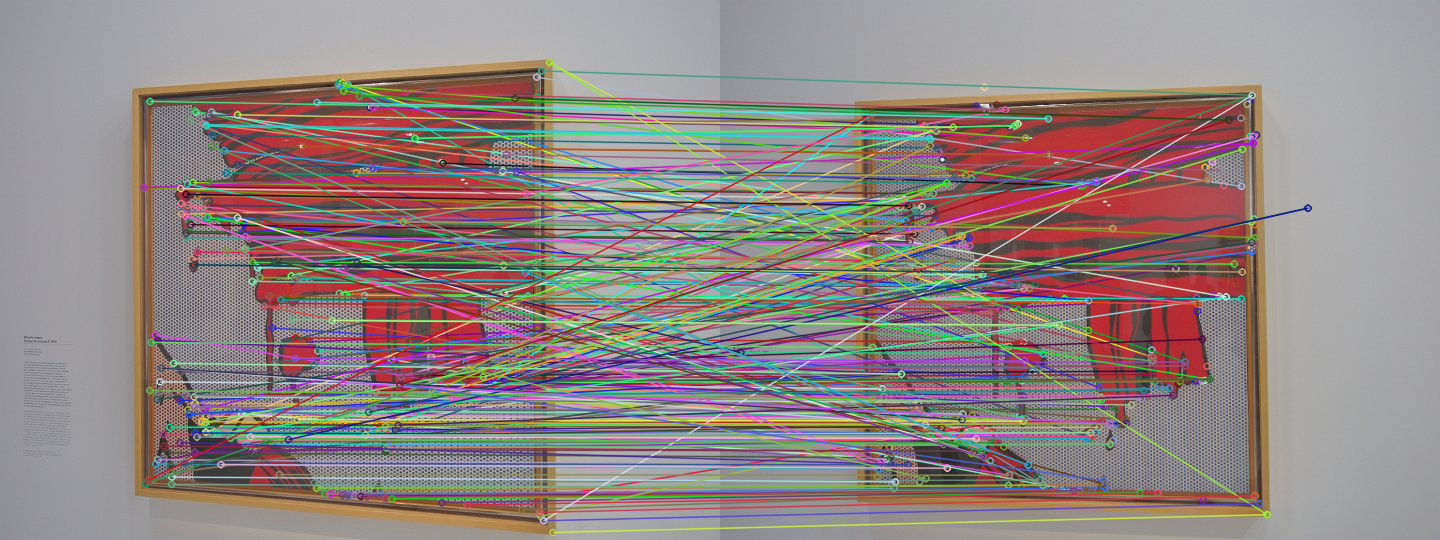
\includegraphics[width=0.75\textwidth]{Fig/sift_raw.png}
  \caption{Paires de descripteurs SIFT entre les deux images avant filtrage par RANSAC}
\end{figure}

\begin{figure}[H]
  \centering
  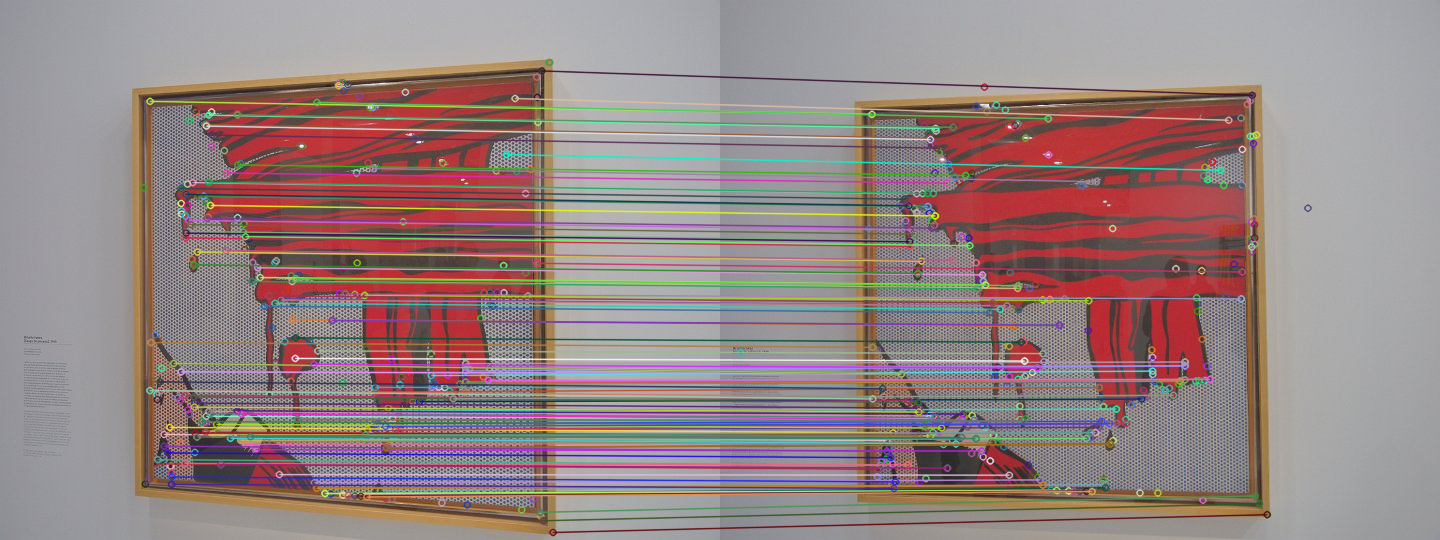
\includegraphics[width=0.75\textwidth]{Fig/sift_ransac.png}
  \caption{Paires de descripteurs SIFT estimés correctes par l'algorithme RANSAC et utilisés pour renconstruire la perspective}
\end{figure}

\begin{figure}[H]
  \centering
  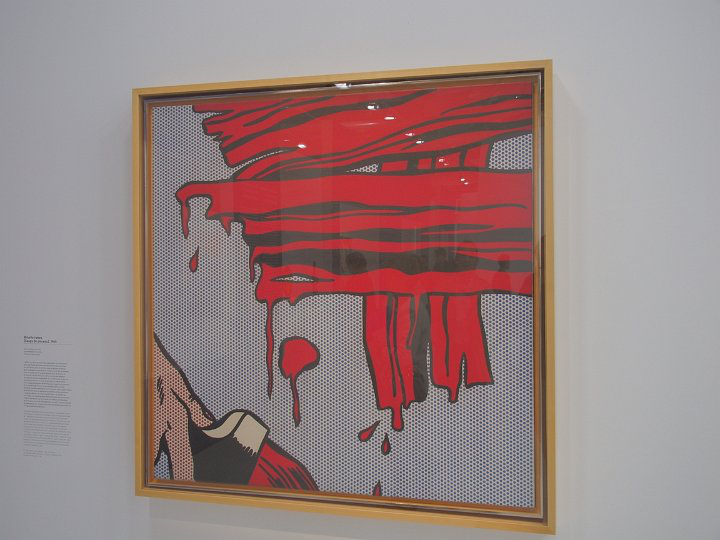
\includegraphics[width=0.30\textwidth]{Fig/working.png}
  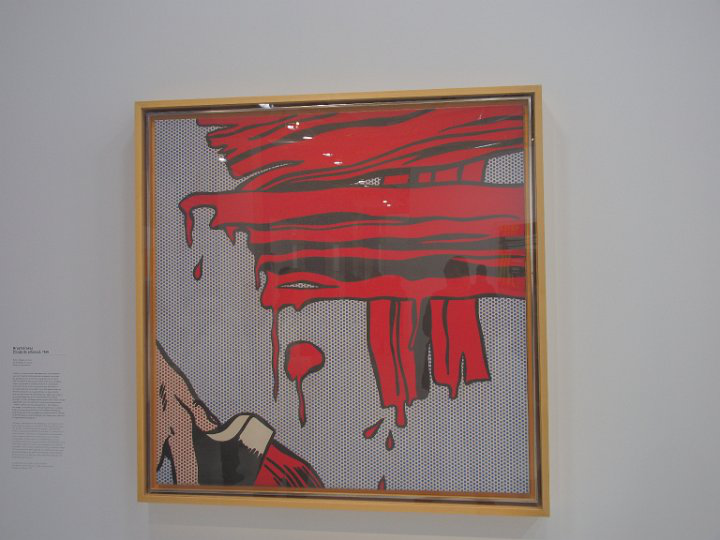
\includegraphics[width=0.30\textwidth]{Fig/reference_image.png}
  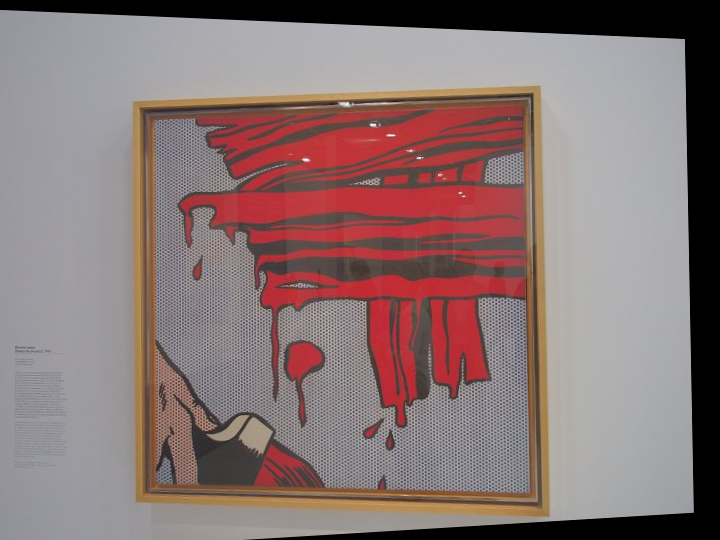
\includegraphics[width=0.30\textwidth]{Fig/fitted.png}

  \caption{A gauche : image de travail, au centre : image de référence, à droite : image de travail après recalage par rapport à l'image de référence. Noter la différence de position des reflets entre l'image de référence et l'image recalée}
\end{figure}

%---------------------------------------------------> SUB SECTION Fusion des images
\subsection{Fusion des images}
Une fois les images recalées, l'étape suivante est de fusionner les images entre elles pour éliminer les reflets. Nous avons testés différentes approches proposées par~\citep{haro2012photographing}, développées ci-après.
%------------------------------------------------------------> SUB SUB SECTION Fusion par minimum
\subsubsection{Fusion par minimum}
Pour cette méthode, nous faisons l'hypothèse que le les reflets ne font qu'ajouter de la luminosité aux différents pixels de l'image, et que les reflets ne peuvent se retrouver dans toutes les images. Dès lors, il suffit de prendre le minimum de chaque canal de couleur pour parvenir à éliminer les reflets.
%------------------------------------------------------------> SUB SUB SECTION Fusion par médianne vectorielle
\subsubsection{Fusion par médiane vectorielle}
Une autre façon consiste à voter, pixel par pixel, pour ce qui devrait être le pixel sans reflet. On suppose ici que le reflet se trouve dans moins de la moitié des images à un endroit donné. Deux méthodes sont alors possibles. On peut prendre la médiane des pixels, canaux de couleurs par canaux de couleurs. Cette méthode, simple et intuitive, à le désavantage, comme la méthode précédente, de mélanger les canaux couleurs d'images différentes, ce qui peut conduire à des couleurs non naturelles. Pour pallier à ce problème, nous avons également implémenté un équivalent de la médiane dans l'espace vectoriel des couleurs ; il s'agit du vecteur minimisant la somme de ses distances $L_1$ aux autres vecteurs. En pratique, nous n'observons pas de différences entre ces deux médianes. 
%------------------------------------------------------------> SUB SUB SECTION Fusion dans l'espace gradient
\subsubsection{Fusion dans l'espace gradient}
Enfin, une méthode décrite dans~\citep{haro2012photographing} permettant de réduire plus les reflets consiste à prendre la médiane vectorielle dans l'espace gradient des images. Pour ce faire, nous calculons les images gradients des images recalées, converties en niveau de gris, et nous en calculons la médiane vectorielle en chaque point. Ensuite, nous construisons les gradients de chaque canal de couleur de l'image fusionnée en prenant, pour chaque point et chaque canal, le gradient de l'image dont la médiane est issue. Ce sont donc bien les gradients des canaux de couleurs qui sont considérés.\\
Lorsque l'on connait le gradient $F$ d'une image, il est possible de la retrouver en minimisant $\min||\mathrm{grad}I - F||$. Ceci se fait grâce à l'équation de Poisson $\Delta I = \mathrm{div}F$. Cette équation est alors résolue, canal par canal, en passant par la transformée de Fourier, s'inspirant de~\citep{morel2010pde}. Rencontrant des difficultés dans cette dernière étape, nous n'avons pas pu terminer cette méthode. Elle donne cependant d'excellents résultats dans~\citep{haro2012photographing}, éliminant certains reflets apparaissant dans une majorité d'images.
%------------------------------------------> SECTION Implémentation
\section{Implémentation}

Pour l'implémentation de la méthode décrite ci-dessus, nous avons choisi des outils C++ accompagné de la librarie OpenCV~\citep{opencv_library} de traitement d'image. La collaboration a été réalisé grâce au gestionnaire de version git. La totalité du code et ses révisions antérieures sont donc disponible sur Github : http://github.com/jcaille/CVCanvas

%------------------------------------------> SECTION Résultats
\section{Résultats}
Les résultats varient peu selon les méthodes (figure~\ref{mediane}). Les médianes permettent de retirer de nombreux artéfacts de reflets, mais ne fonctionnent pas là où une majorité d'images présentent des artéfacts. Les méthodes de médiane, canal par canal ou globale, donnent les mêmes résultats sur les exemples que nous avons essayés.
\begin{figure}
\centering
\begin{minipage}{0.6\linewidth}
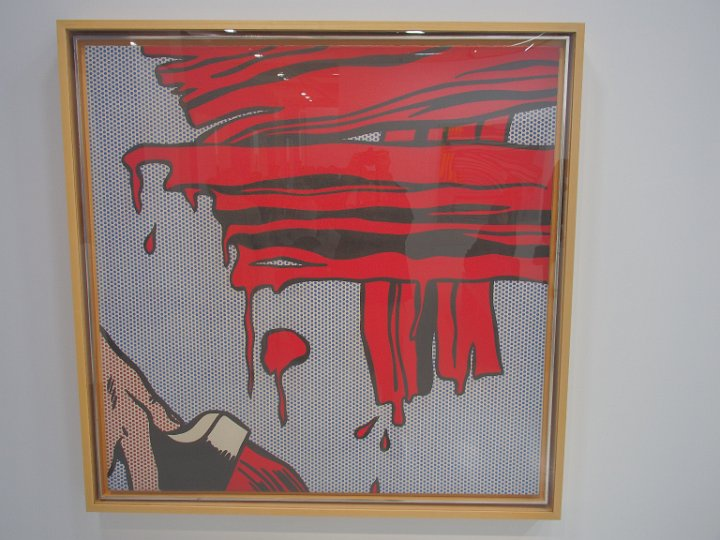
\includegraphics[width=\textwidth]{Fig/reference.jpg}
\end{minipage}
\begin{minipage}{0.6\linewidth}
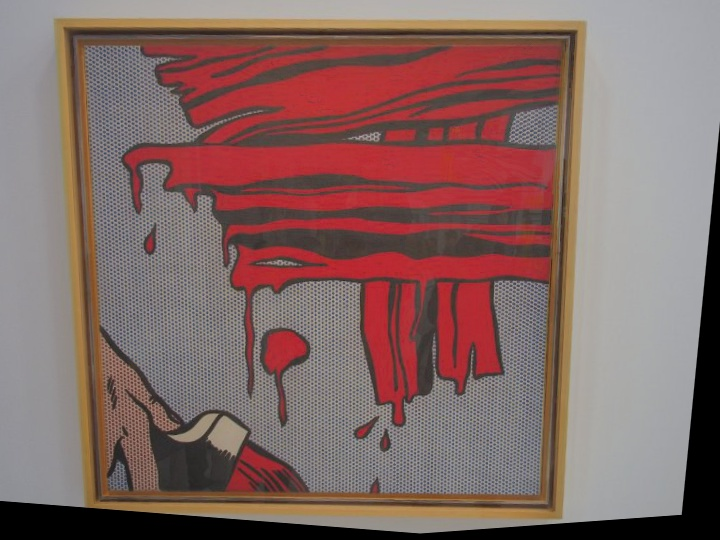
\includegraphics[width=\textwidth]{Fig/merge_min.jpg}
\end{minipage}
\begin{minipage}{0.6\linewidth}
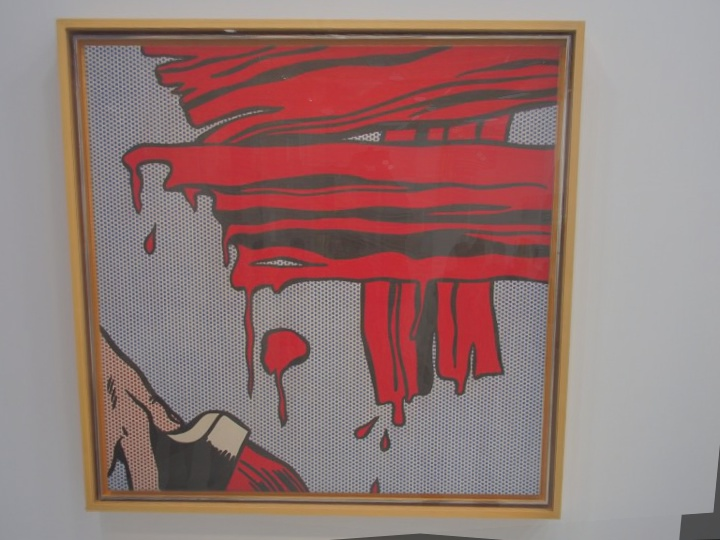
\includegraphics[width=\textwidth]{Fig/merge_median.jpg}
\end{minipage}
\caption{Correction des artéfacts. De haut en bas : image de référence, puis corrigée avec les méthodes du minimum et de la médiane.}
\label{mediane}
\end{figure} 
%------------------------------------------> SECTION Améliorations possibles
\section{Améliorations possibles}

Plusieurs amélioration de l'algorithme sont envisageables. Si les images obtenues sont de bonne qualité, l'algorithme ne sait pas faire la différence entre les zones de la peinture et les zones extérieures (cadre, mur, paysage, ...), dans lesquelles la fusion est effectuée alors qu'elle n'a pas de sens. Une possibilité pour détecter ces zones et de segmenter l'image de référence (par exemple en utilisant des snakes quadrangulaires) entre un "intérieur" sur lequel la fusion serait effectué et un extérieur sur lequel on garderait le contenu d'origine. Pour s'aider dans cette segmentation, nous pourrions utiliser les informations des autres photos du tableau.

De plus, l'algorithme que nous avons développé (en particulier la partie de fusion) n'est pas de fait résistant aux changements de contrastes en général. Une idée pour corriger ce défaut serait d'égaliser les histogrammes les différentes images (de préférence en limitant cette égalisation à la zone "intérieur" du tableau).
\bibliographystyle{plain}
\bibliography{QUEEN}
\end{document}
